\chapter{Theory}
This package contains a few simple two-dimensional geometric objects. The geometric objects are defined by a sufficient amount of points. Further information can be found in~\cite{geometry}.
\section{Points}
A point $\mathbf{p}$ in a two-dimensional space can be described by its Cartesian coordinates
\begin{align}
    \mathbf{p} = \begin{pmatrix} x \\ y \end{pmatrix}.
\end{align}
If two points $\mathbf{p}_1$ and $\mathbf{p}_2$ are defined, we can connect those points using the connection vector $\mathbf{c}$ (see Fig.~\ref{fig:distance}), which can be calculated by s the individual entries of $\mathbf{p}_1$ and $\mathbf{p}_2$
\begin{align}
    \mathbf{c}  = \mathbf{p}_1 - \mathbf{p}_2 = \begin{pmatrix} x_1 \\ y_1 \end{pmatrix} - \begin{pmatrix} x_2 \\ y_2 \end{pmatrix}
\end{align}

\begin{figure}[h]
    \centering
    \begin{tikzpicture}
        %KOS
        \draw[->,thick,black] (0,0) -- (0,3.5);
        \draw (0.2,3.7) node [fill=white] {$y$};
        \draw[->,thick,black] (0,0) -- (5.5,0);
        \draw (5.7,0.2) node [fill=white] {$x$};
        
        \fill[black] (1,1) circle (2pt);
        \fill[black] (3,2) circle (2pt);
        
        \draw[->,thin,blue] (1,1) -- (3,2);
        \draw (2,1.8) node [fill=white] {$\mathbf{c}$};
    \end{tikzpicture}
    \caption{Distance between two points.}
    \label{fig:distance}
\end{figure}
Calculating the norm of $\mathbf{c}$
\begin{align}
    d = ||\mathbf{c}|| = || \begin{pmatrix} c_x \\ c_y \end{pmatrix} || = \sqrt{c_x^2 + c_y^2}
\end{align}
yields the distance $d$ between both points. In the following sections the distance between two points is indicated as $d(\mathbf{p_1},\mathbf{p_2})$

\section{Circle}
A circle is defined by its center point $\mathbf{p}_1$ and radius $r$. Depending on $r$ the surface area $a$ of the circle can be calculated as
\begin{align}
    a =\pi r^2.
\end{align}
Furthermore the perimeter $p$ of the circle is calculated via
\begin{align}
    p = 2 \pi r.
\end{align}
Both measurements are independent of $\mathbf{p}_1$.
\section{Rectangle}
A rectangle is defined by at least two corner points $\mathbf{p}_1$ and $\mathbf{p_2}$. Since the sides of the rectangle intersect each other at $90^{\circ}$, and for this package it is assumed that the sides are parallel to the Cartesian axes, the structure of the rectangle is implicitly given by just specifying two corner points of non adjacent corners, see Fig.~\ref{fig:rectangle}.
\begin{figure}[hbt]
    \centering
    \begin{tikzpicture}
        %KOS
        \draw[->,thick,black] (0,0) -- (0,3.5);
        \draw (0.2,3.7) node [fill=white] {$y$};
        \draw[->,thick,black] (0,0) -- (5.5,0);
        \draw (5.7,0.2) node [fill=white] {$x$};
        
        \draw[-,thin,blue] (1,1) -- (1,3);
        \draw[-,thin,blue] (1,1) -- (4,1);
        \draw[-,thin,blue] (4,3) -- (1,3);
        \draw[-,thin,blue] (4,3) -- (4,1);
        
        \draw (2.5,3.3) node [fill=white] {$w$};
        \draw (0.7,2) node [fill=white] {$h$};
        
        \draw (0.8,0.8) node [fill=white] {$\mathbf{p_1}$};
        \fill[black] (1,1) circle (2pt);
        \draw (4.2,3.2) node [fill=white] {$\mathbf{p_2}$};
        \fill[black] (4,3) circle (2pt);
        
    \end{tikzpicture}
    \caption{Definition of a Rectangle.}
    \label{fig:rectangle}
\end{figure}
In order to calculate the perimeter or the surface area of the rectangle, we need to calculate the height $h$ and the width $w$ of the rectangle as
\begin{align}
    h &= |p_{1y} - p_{2y}| \\
    w &= |p_{1x} - p_{2x}|.
\end{align}
Since the order of the corner points could be switched, we take the absolute value of both measurements. With known height and width, the area $a$ can be calculated as 
\begin{align}
    a = h \cdot w
\end{align}
and the perimeter $p$ as
\begin{align}
    p = 2h + 2w.
\end{align}
\section{Triangle}
A triangle is defined by three corner points $\mathbf{p}_1 - \mathbf{p}_3$, see Fig.~\ref{fig:triangle}. Note that a specific ordering of those points is not required.
\begin{figure}[hbt]
    \centering
    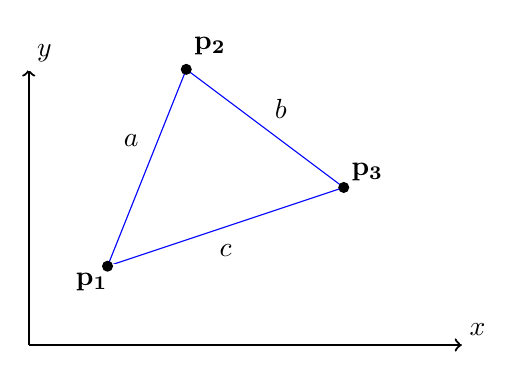
\begin{tikzpicture}
        %KOS
        \draw[->,thick,black] (0,0) -- (0,3.5);
        \draw (0.2,3.7) node [fill=white] {$y$};
        \draw[->,thick,black] (0,0) -- (5.5,0);
        \draw (5.7,0.2) node [fill=white] {$x$};
        
        \draw[-,thin,blue] (1,1) -- (2,3.5);
        \draw (1.3,2.6) node [fill=white] {$a$};
        \draw[-,thin,blue] (2,3.5) -- (4,2);
        \draw (3.2,3) node [fill=white] {$b$};
        \draw[-,thin,blue] (4,2) -- (1,1);
        \draw (2.5,1.2) node [fill=white] {$c$};
        
        \draw (0.8,0.8) node [fill=white] {$\mathbf{p_1}$};
        \fill[black] (1,1) circle (2pt);
        \draw (2.3,3.8) node [fill=white] {$\mathbf{p_2}$};
        \fill[black] (2,3.5) circle (2pt);
        \draw (4.3,2.2) node [fill=white] {$\mathbf{p_3}$};
        \fill[black] (4,2) circle (2pt);
        
    \end{tikzpicture}
    \caption{Definition of a Triangle.}
    \label{fig:triangle}
\end{figure}
To calculate the surface area $a$ and the perimeter $b$, we need to calculate the side lengths of the triangle first. We define the side lengths $a,b,c$ as
\begin{align}
    a = d(\mathbf{p}_1, \mathbf{p}_2),\\
    b = d(\mathbf{p}_2, \mathbf{p}_3),\\
    c = d(\mathbf{p}_3, \mathbf{p}_1).
\end{align}
We can then calculate the surface area $a$ of an arbitrary triangle as 
\begin{align}
    a = \sqrt{s(s-a)(s-b)(s-c)}
\end{align}
with
\begin{align}
    s = \frac{a+b+c}{2}.
\end{align}
Further, the perimeter is calculated as
\begin{align}
    p = 2s = a+b+c.
\end{align}